\documentclass[10pt]{beamer}

% --- Tema i Estètica ---
\usetheme{Madrid}
\usecolortheme{whale}

% --- Paquets ---
\usepackage[utf8]{inputenc}
\usepackage[T1]{fontenc}
\usepackage[english]{babel}
\usepackage{listings}
\usepackage{graphicx}
\usepackage{booktabs}
\usepackage[style=apa,backend=biber]{biblatex}
\addbibresource{referencesforrepli.bib}

% Configuració de Codi R
\lstset{
	language=R,
	breaklines=true,
	basicstyle=\ttfamily\tiny,
	keywordstyle=\color{blue}
}

% --- Informació del Títol ---
\title[Replication: Brexit in NI]{The past, Brexit, and the future in Northern Ireland: a quasi-experiment}
\subtitle{Replication and Extension (Assignment POP77082)}
\author{Rubèn Llorens Poblador}
\date{April 1, 2026}

\begin{document}
	
	% 1. Portada
	\begin{frame}
		\titlepage
	\end{frame}
	
	% 2. Índex
	\begin{frame}{Outline}
		\tableofcontents
	\end{frame}
	
	\section{Original Study}
	
	\begin{frame}{The Original Study: Research Question}
		\begin{itemize}
			\item \textbf{Authors:} Godefroidt, Dyrstad \& Bakke (2023).
			\item \textbf{Goal:} Test the effect of the Brexit referendum outcome on:
			\begin{enumerate}
				\item Perceptions of the causes of \textit{The Troubles}.
				\item Constitutional preferences for Northern Ireland.
			\end{enumerate}
			\item \textbf{Mechanism:} Brexit as a key factor that reactivates memories of political and economic instability.
		\end{itemize}
	\end{frame}
	
	\begin{frame}{Quasi-Experimental Design}
		\begin{block}{Exogenous Shock}
			The referendum (June 23, 2016) took place \textbf{during} the fieldwork of the \textit{Post-conflict Attitudes for Peace} (PAP) survey.
		\end{block}
		\begin{itemize}
			\item \textbf{Control Group:} Surveyed before June 23.
			\item \textbf{Treatment Group:} Surveyed after the "Leave" outcome was known.
			\item \textbf{Method:} Entropy Balancing (EB) to ensure comparability between groups.
		\end{itemize}
	\end{frame}
	
	\section{Replication Results}
	
	\begin{frame}{Replication: Perception of Causes (Fig 1)}
		\begin{columns}
			\begin{column}{0.5\textwidth}
				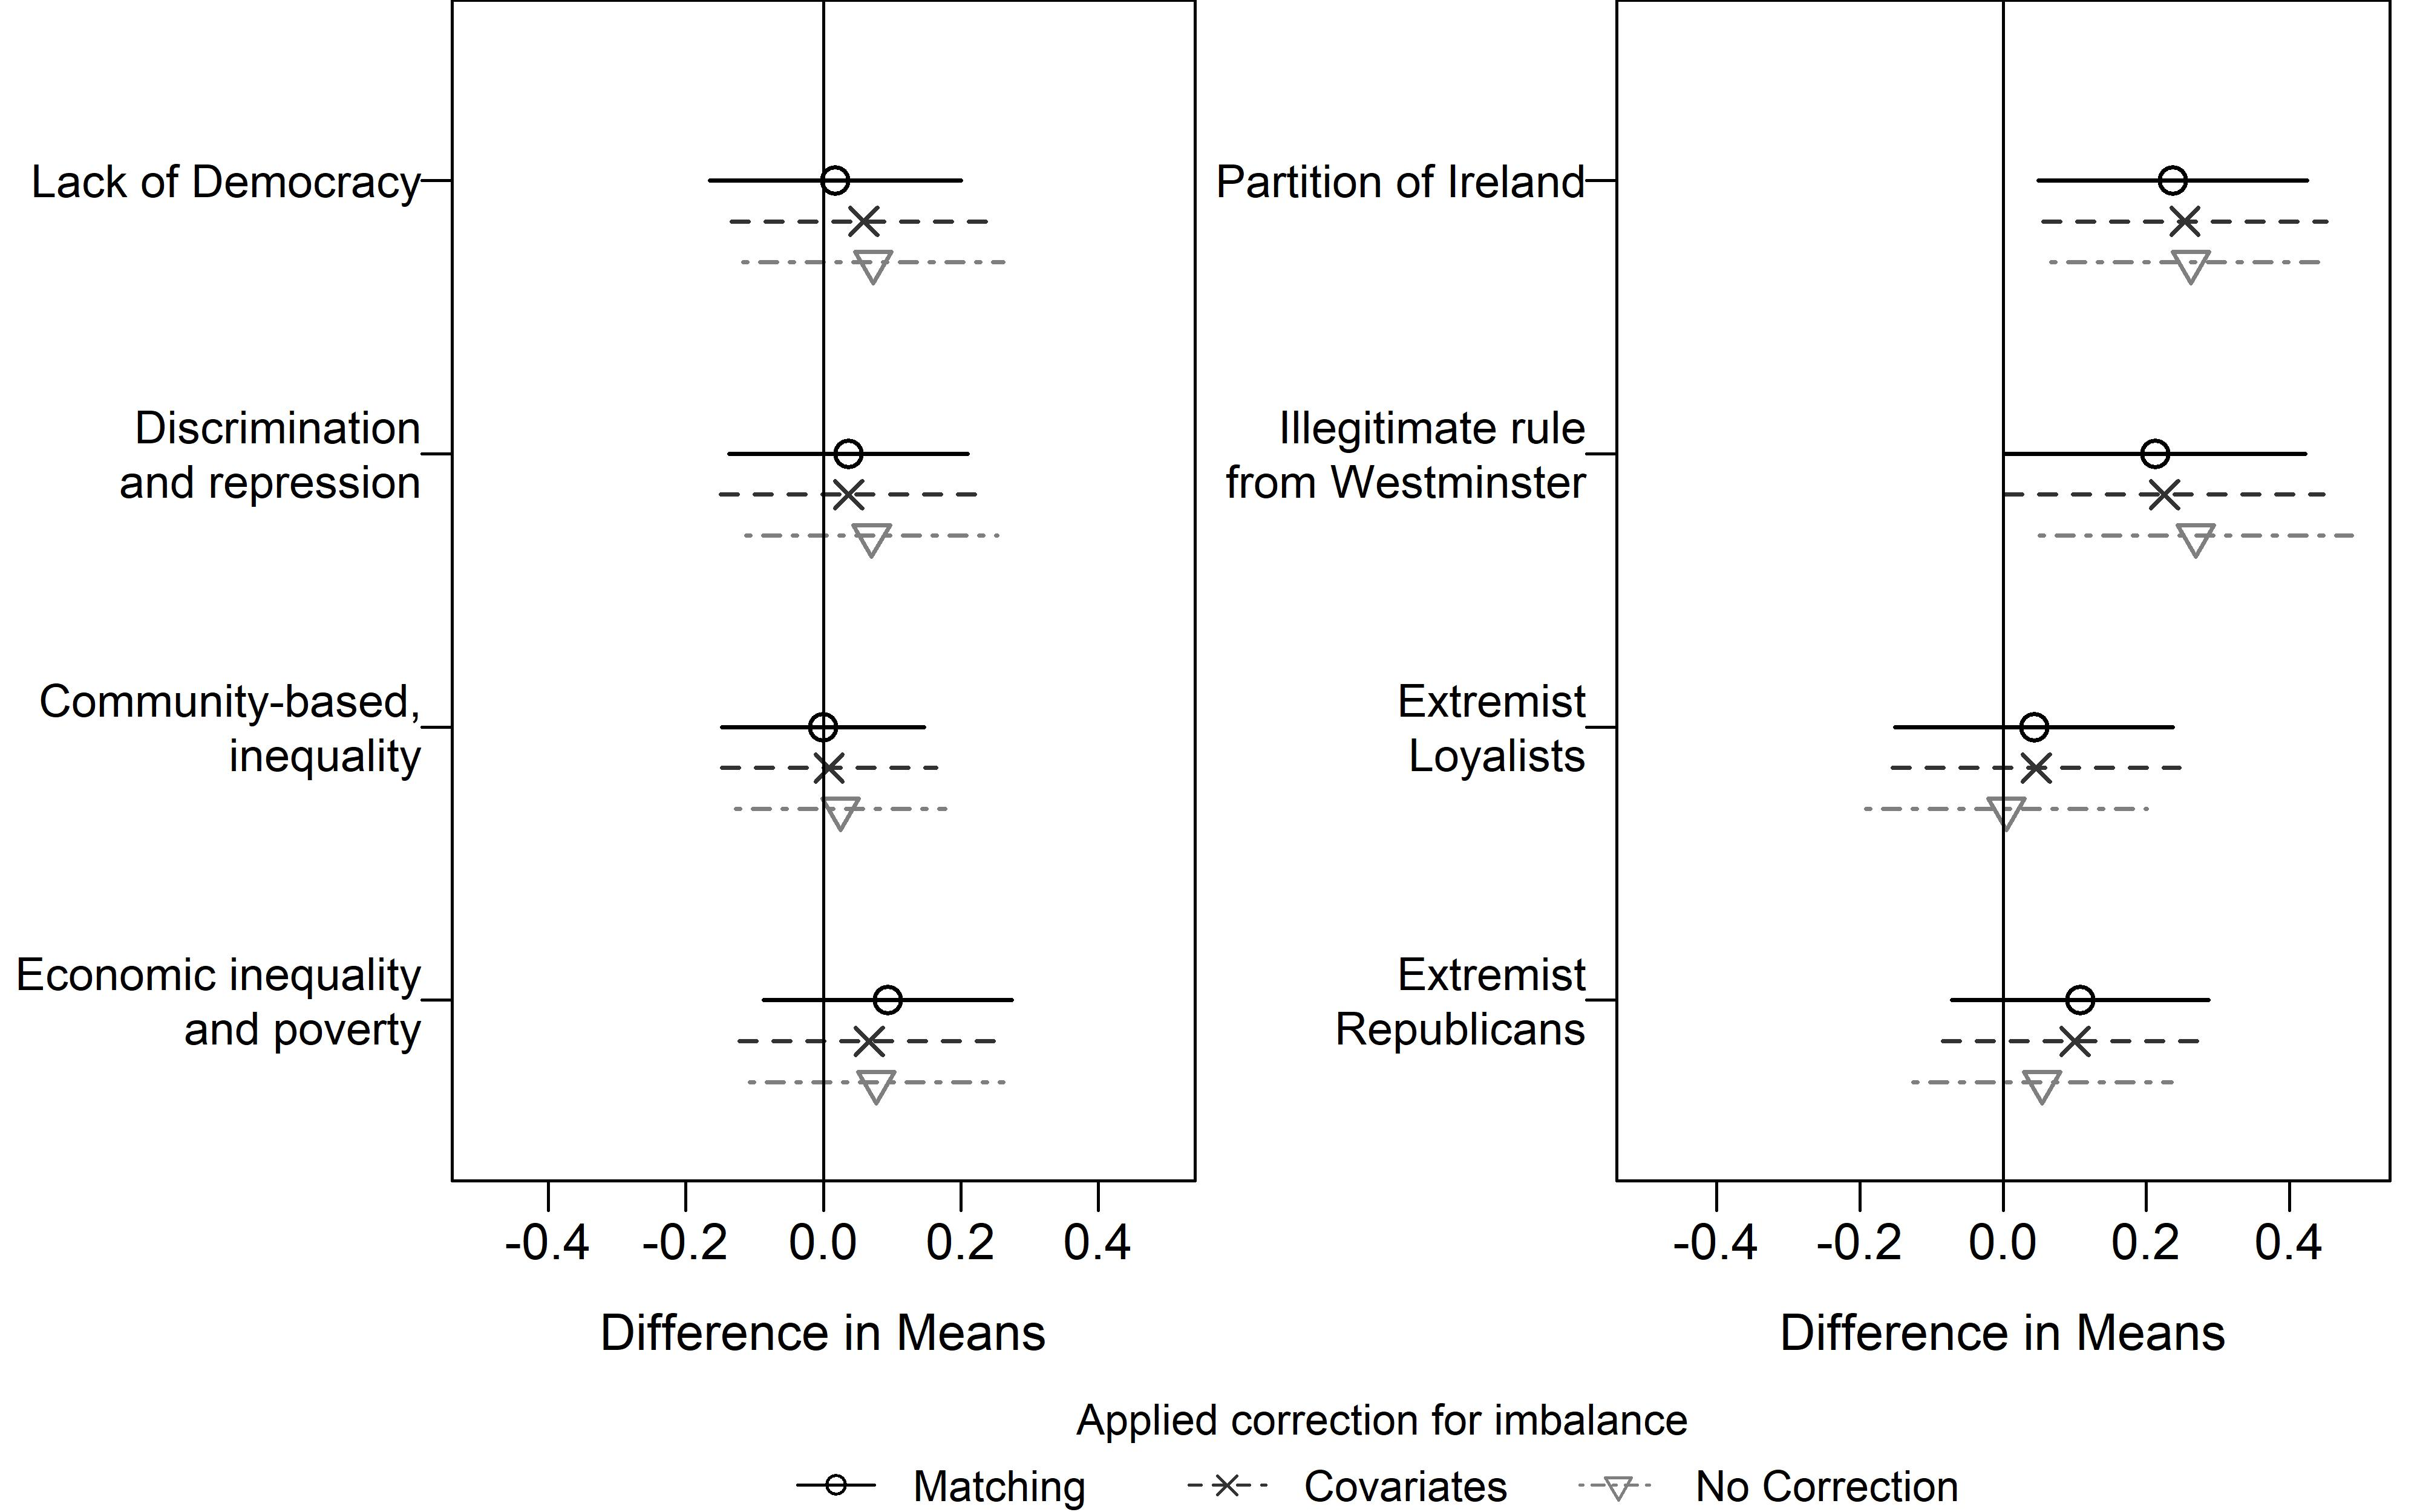
\includegraphics[width=\textwidth]{Fig1.jpeg}
			\end{column}
			\begin{column}{0.5\textwidth}
				\small
				\begin{itemize}
					\item Significant increase in the perceived importance of \textbf{Westminster rule} and the \textbf{partition of Ireland}.
					\item Robust results across different model specifications (Matching, Covariates, No correction).
				\end{itemize}
			\end{column}
		\end{columns}
	\end{frame}
	
	\begin{frame}{Replication: Constitutional Preferences (Fig 2 \& 3)}
		\begin{itemize}
			\item \textbf{Irish Unification:} +9 percentage point increase.
			\item \textbf{Remain in UK:} -13 percentage point drop.
			\item \textbf{Independence:} No significant change.
		\end{itemize}
		\begin{center}
	\begin{figure}[h]
	\centering
	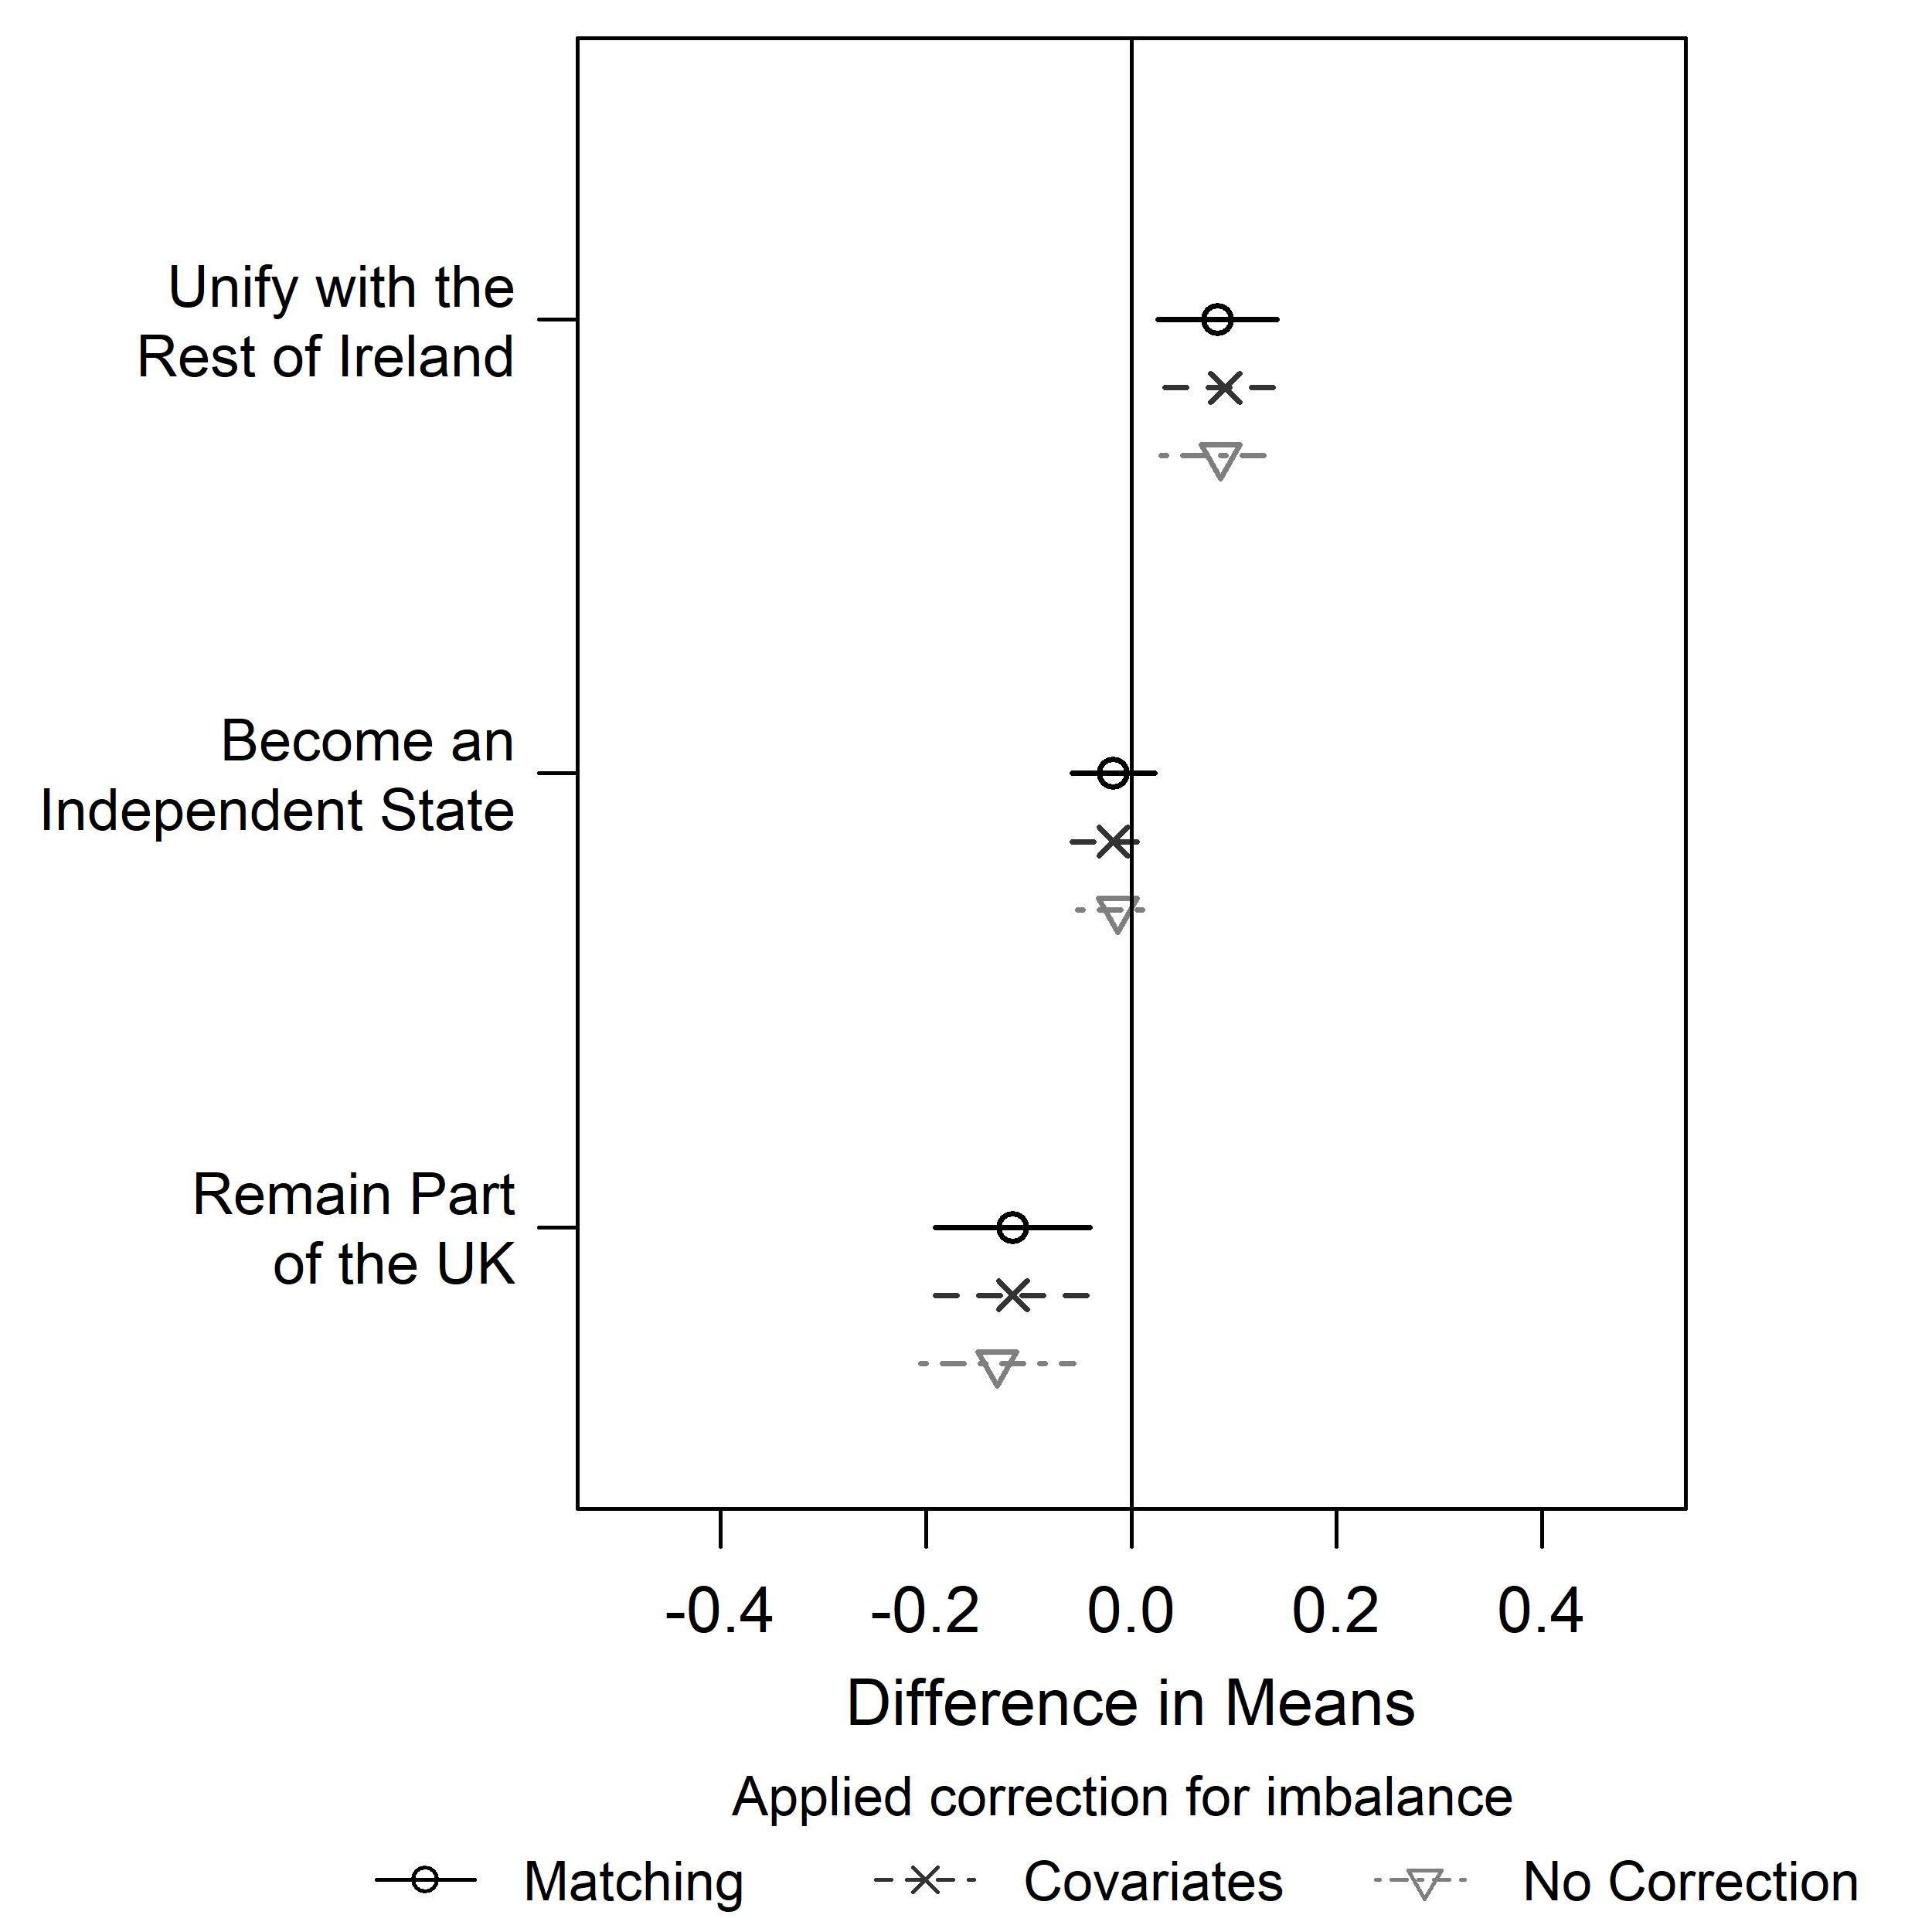
\includegraphics[width=0.5\textwidth]{Fig3.jpeg}
	\label{fig:meva_figura_3}
\end{figure}
		\end{center}
	\end{frame}
	

	
	\section{My Contribution: Extensions}
	
	\begin{frame}{The Extension: Heterogeneous Effects}
		\textbf{Research Question:} Is the Brexit effect uniform or does it vary by demographic profile?
		\vfill
		\begin{block}{Interaction Models (GLM Logit)}
			$$ \text{Unification} \sim \text{Referendum} \times \text{Moderator} + \text{Controls} $$
		\end{block}
		\vfill
		\begin{itemize}
			\item \textbf{Moderator 1:} Age Cohorts (18-25, 26-45, Over 45).
			\item \textbf{Moderator 2:} Exposure to the Troubles (Victims vs Non-victims).
			\item \textbf{Moderator 3:} Gender (Male vs Female).
		\end{itemize}
	\end{frame}
	
	\begin{frame}{Extension 1: Age Cohorts}
		\begin{columns}
			\begin{column}{0.5\textwidth}
				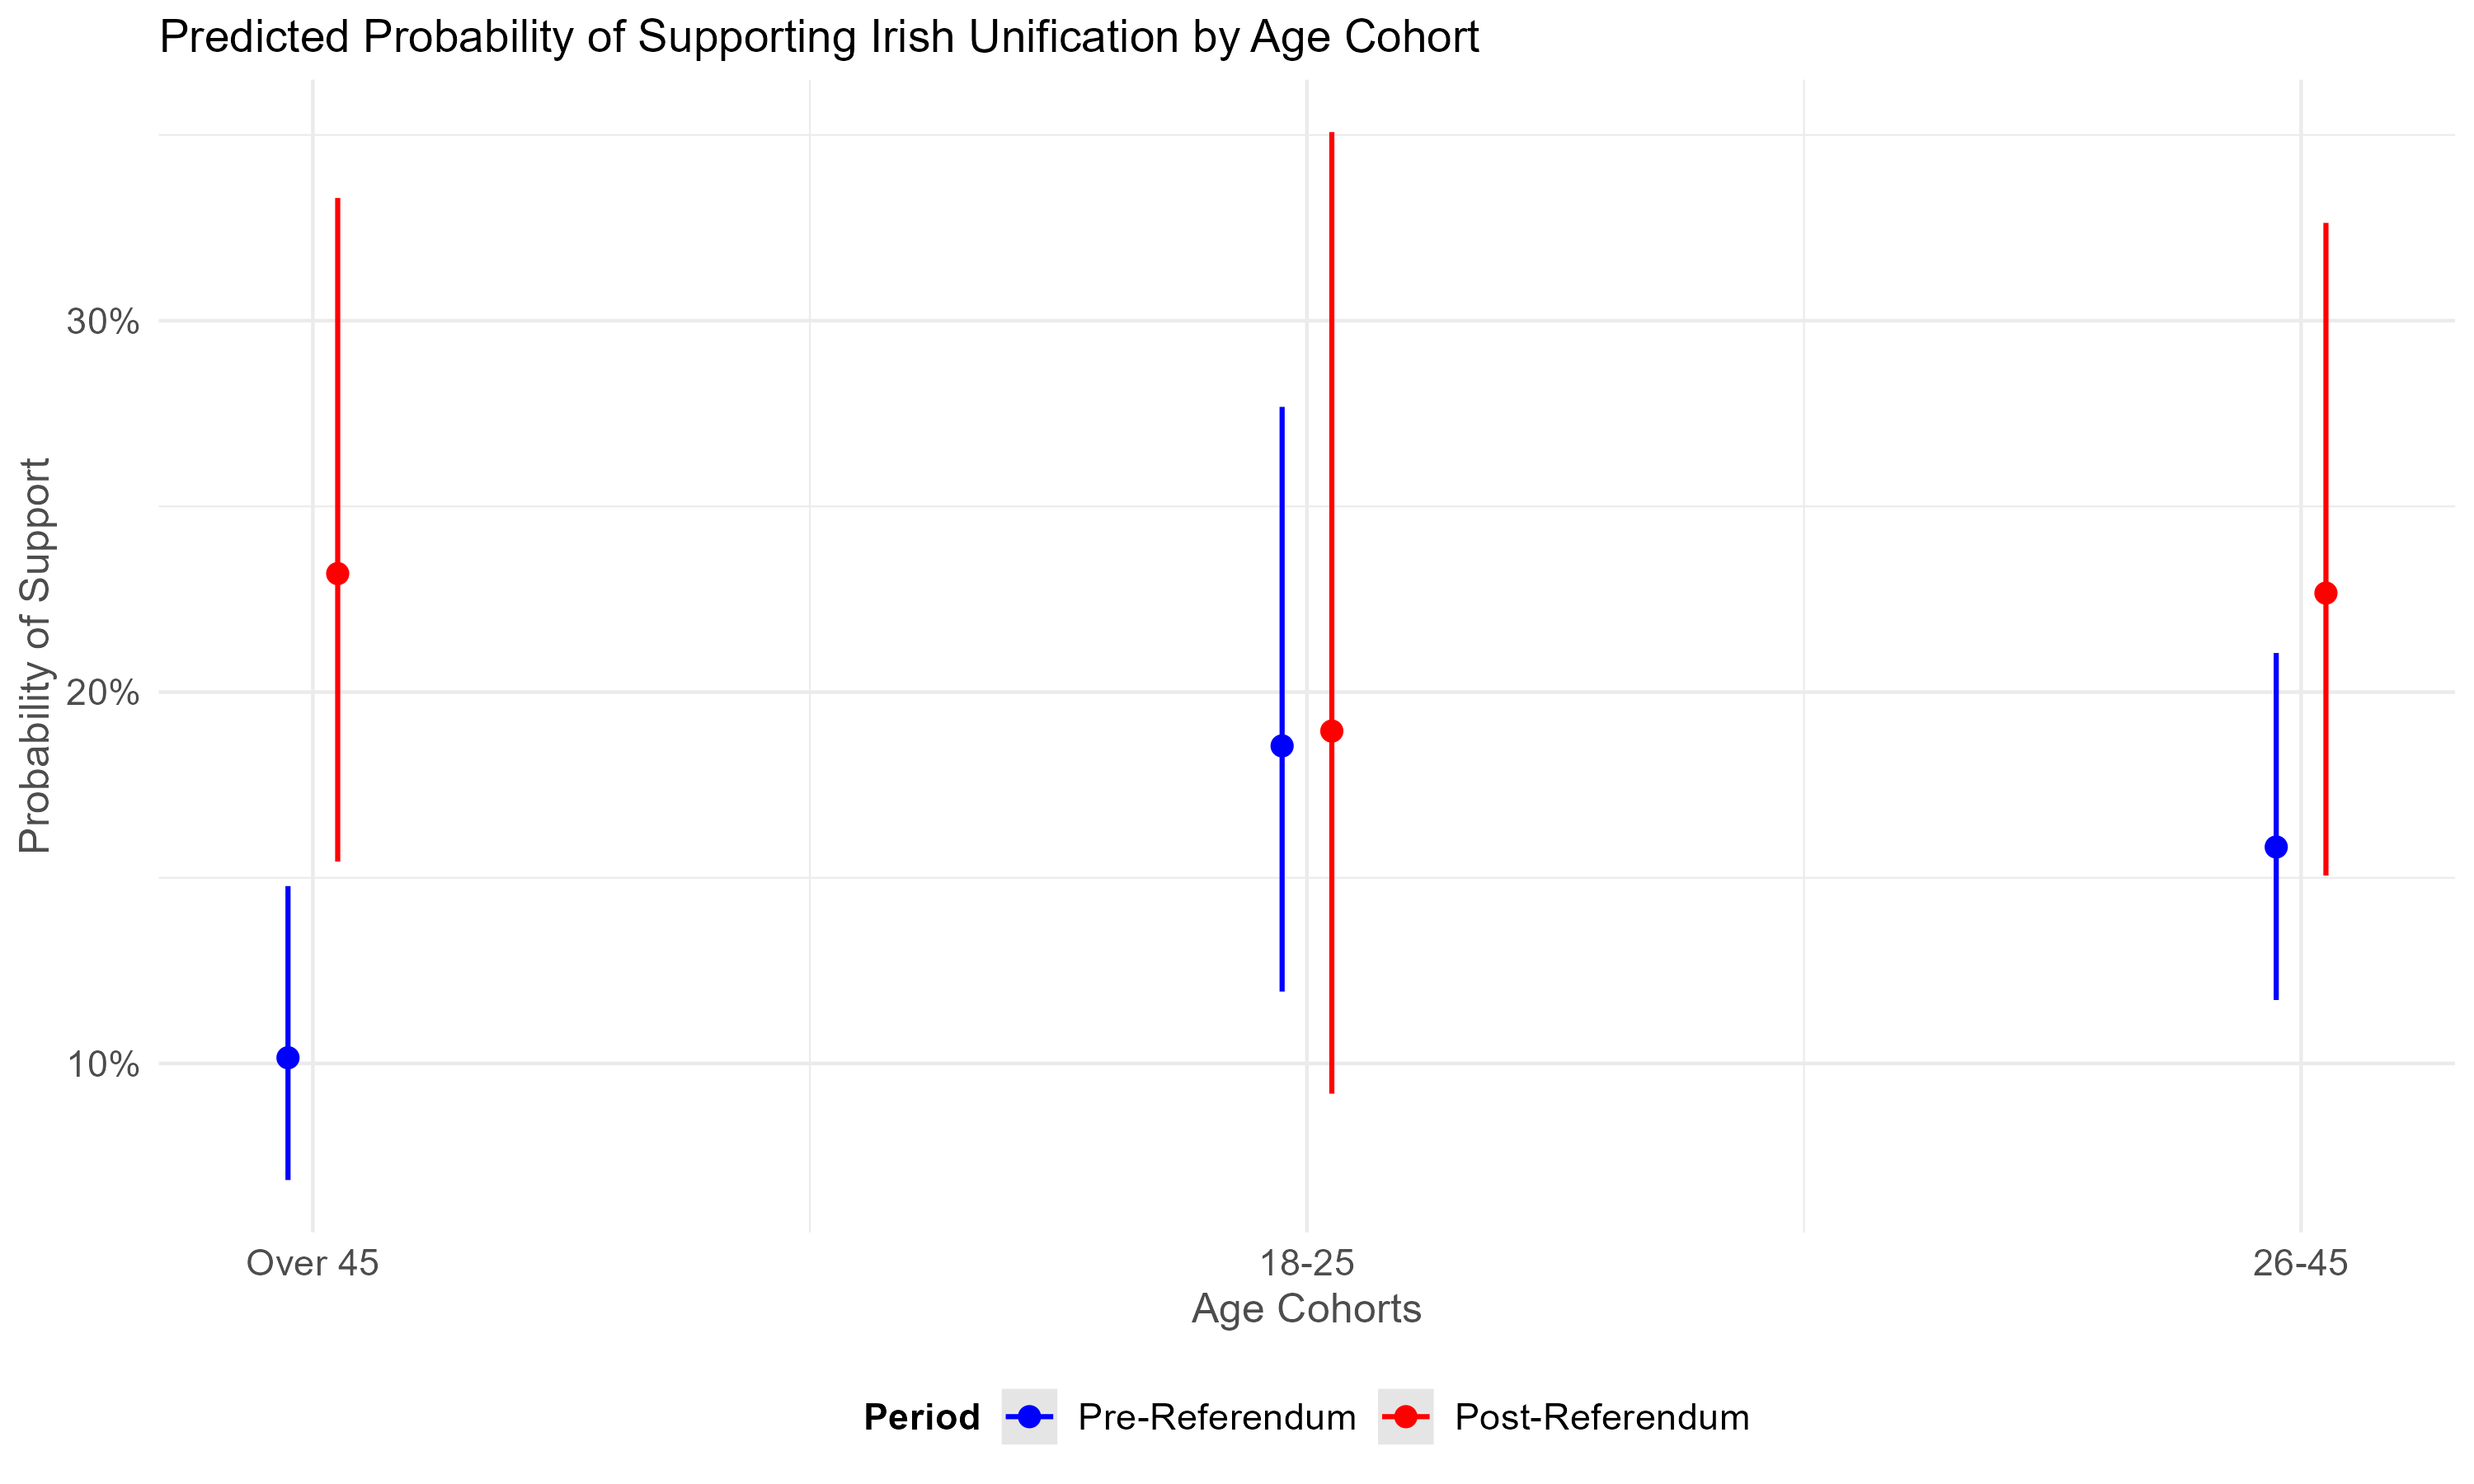
\includegraphics[width=\textwidth]{plot_ext1.png}
			\end{column}
			\begin{column}{0.5\textwidth}
				\begin{itemize}
					\item \textbf{Result:} Non-significant interaction.
					\item \textbf{Interpretation:} Brexit acted as a \textbf{universal systemic shock}.
					\item The "jump" is parallel across all cohorts, though the Over 45s show a more precise doubling of support.
				\end{itemize}
			\end{column}
		\end{columns}
	\end{frame}
	
	\begin{frame}{Extension 2: Exposure to the Troubles}
		\begin{columns}
			\begin{column}{0.5\textwidth}
				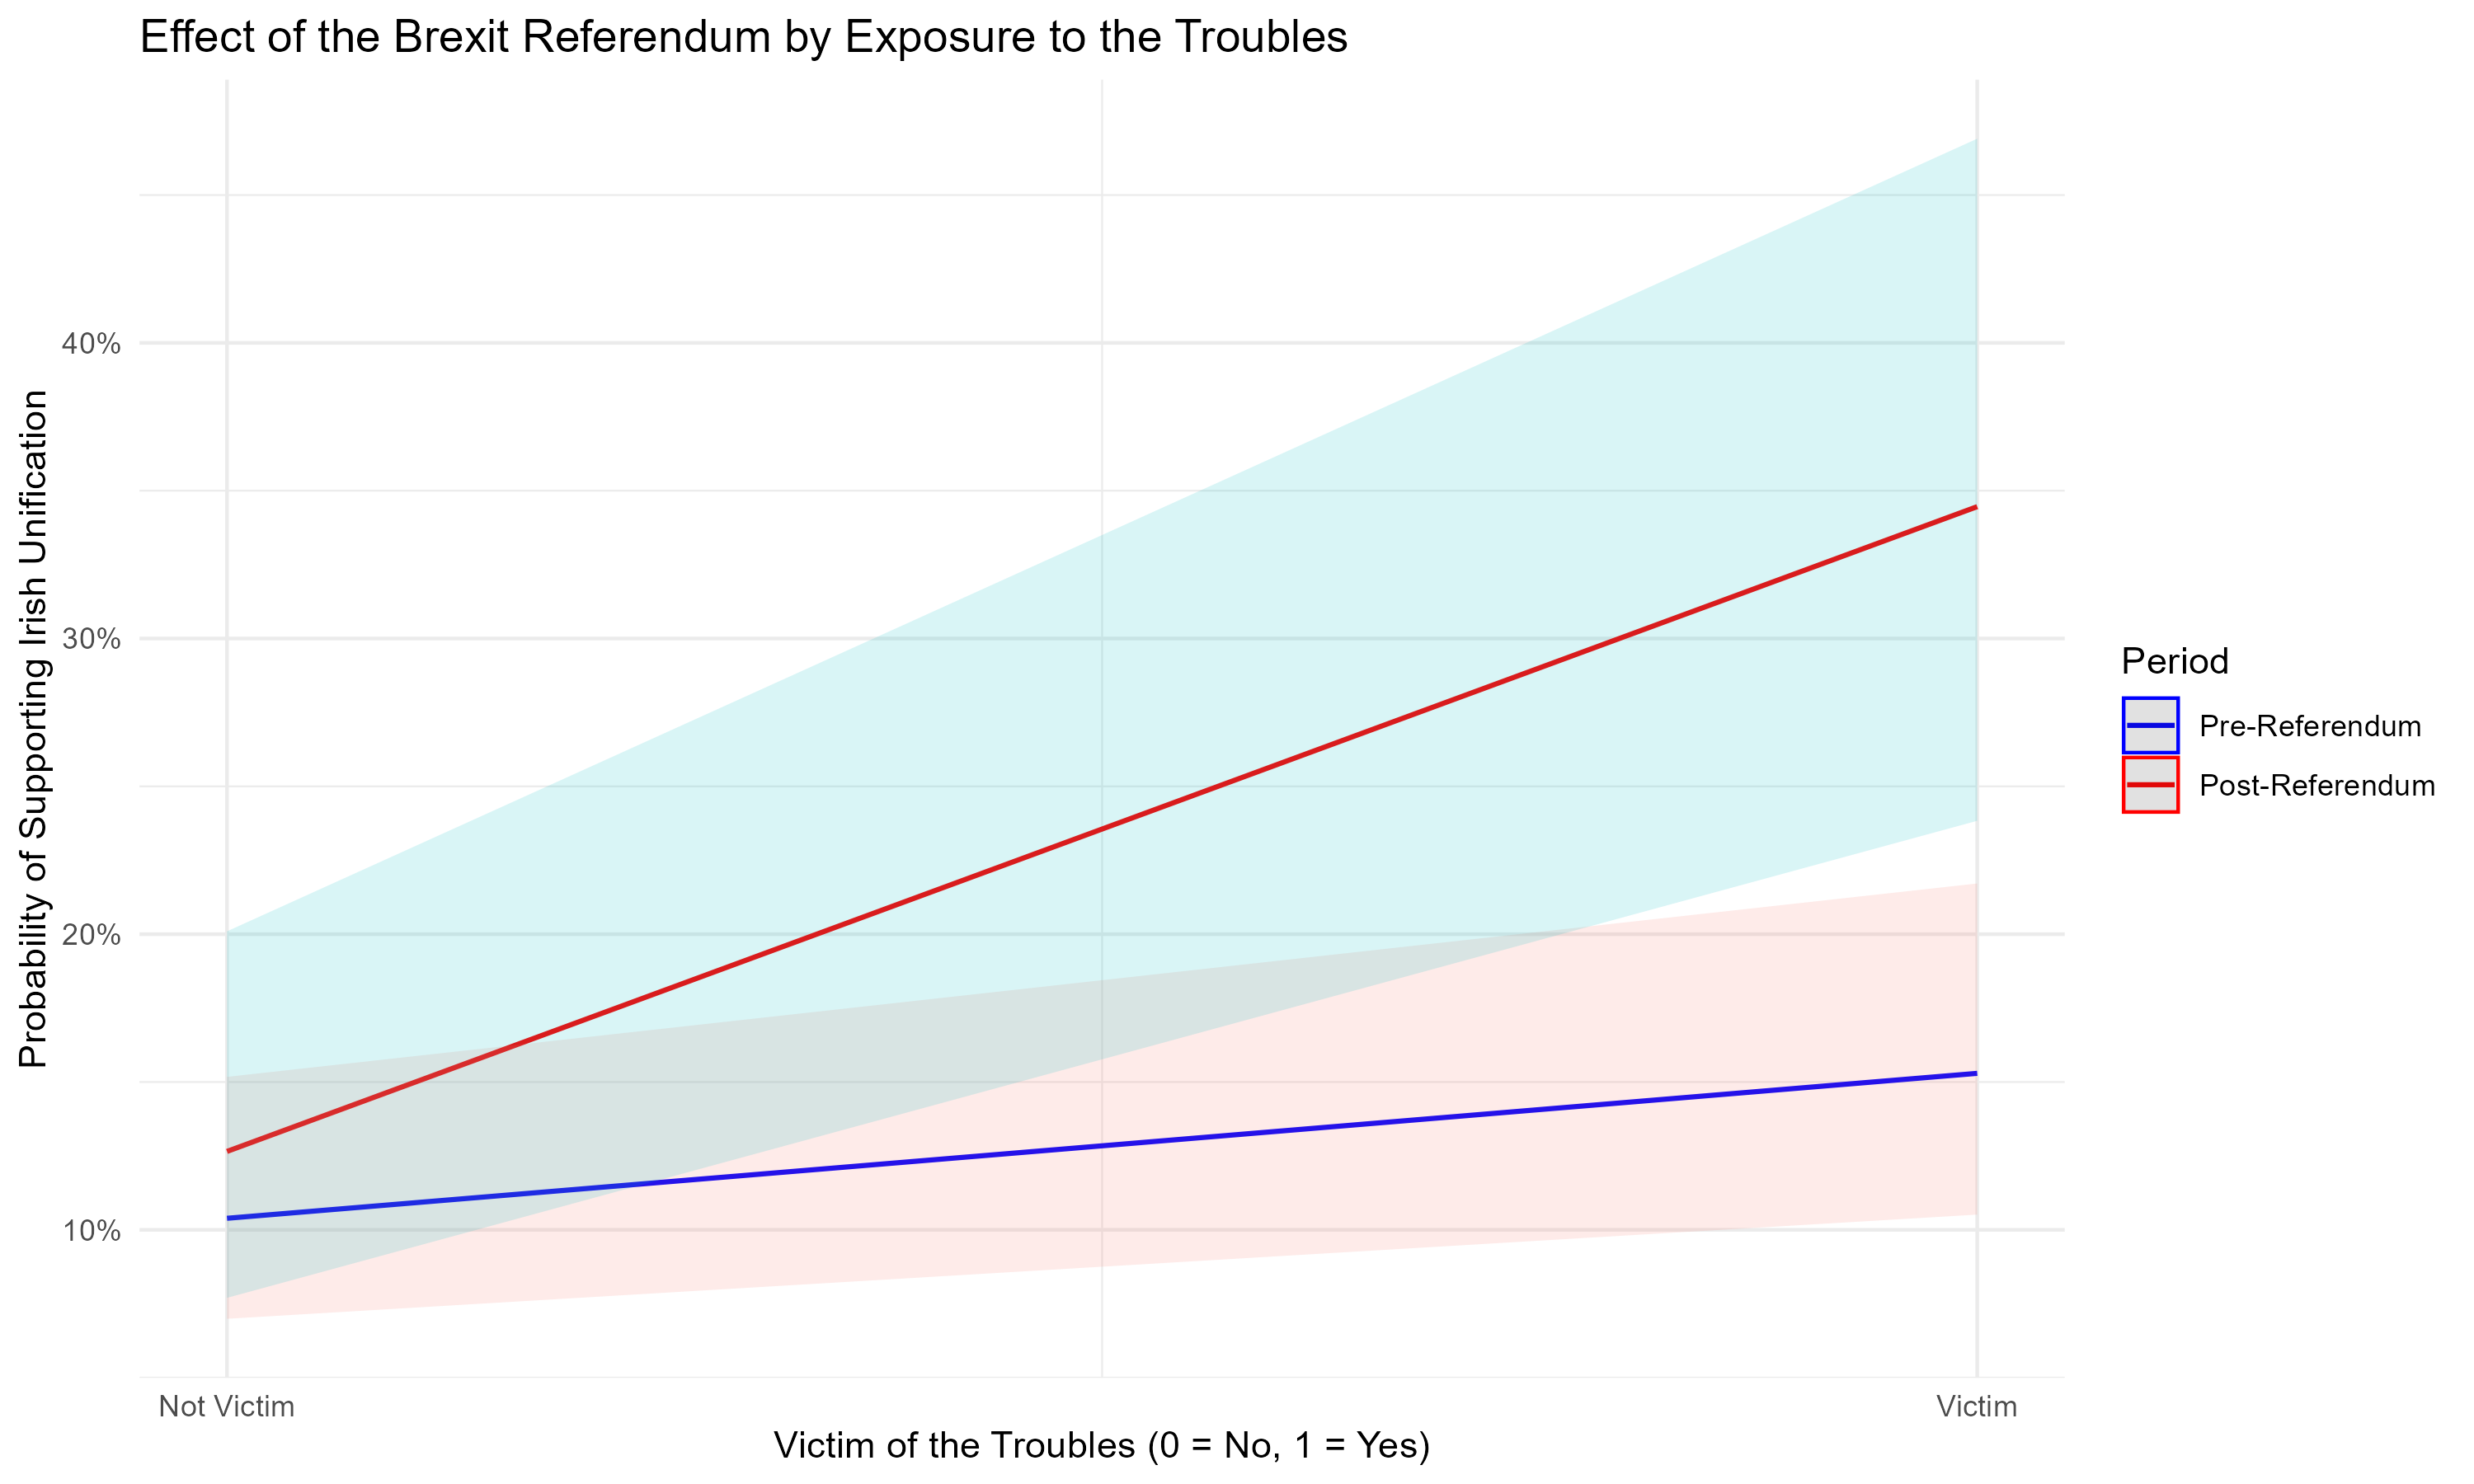
\includegraphics[width=\textwidth]{plot_ext2.png}
			\end{column}
			\begin{column}{0.5\textwidth}
				\begin{itemize}
					\item \textbf{Result:} Significant interaction ($p < 0.05$).
					\item \textbf{Interpretation:} The referendum had a \textbf{stronger effect on victims}.
					\item Personal trauma acts as a catalyst for political change when stability is threatened.
				\end{itemize}
			\end{column}
		\end{columns}
	\end{frame}
	
	\begin{frame}{Extension 3: Gender}
		\begin{columns}
			\begin{column}{0.5\textwidth}
				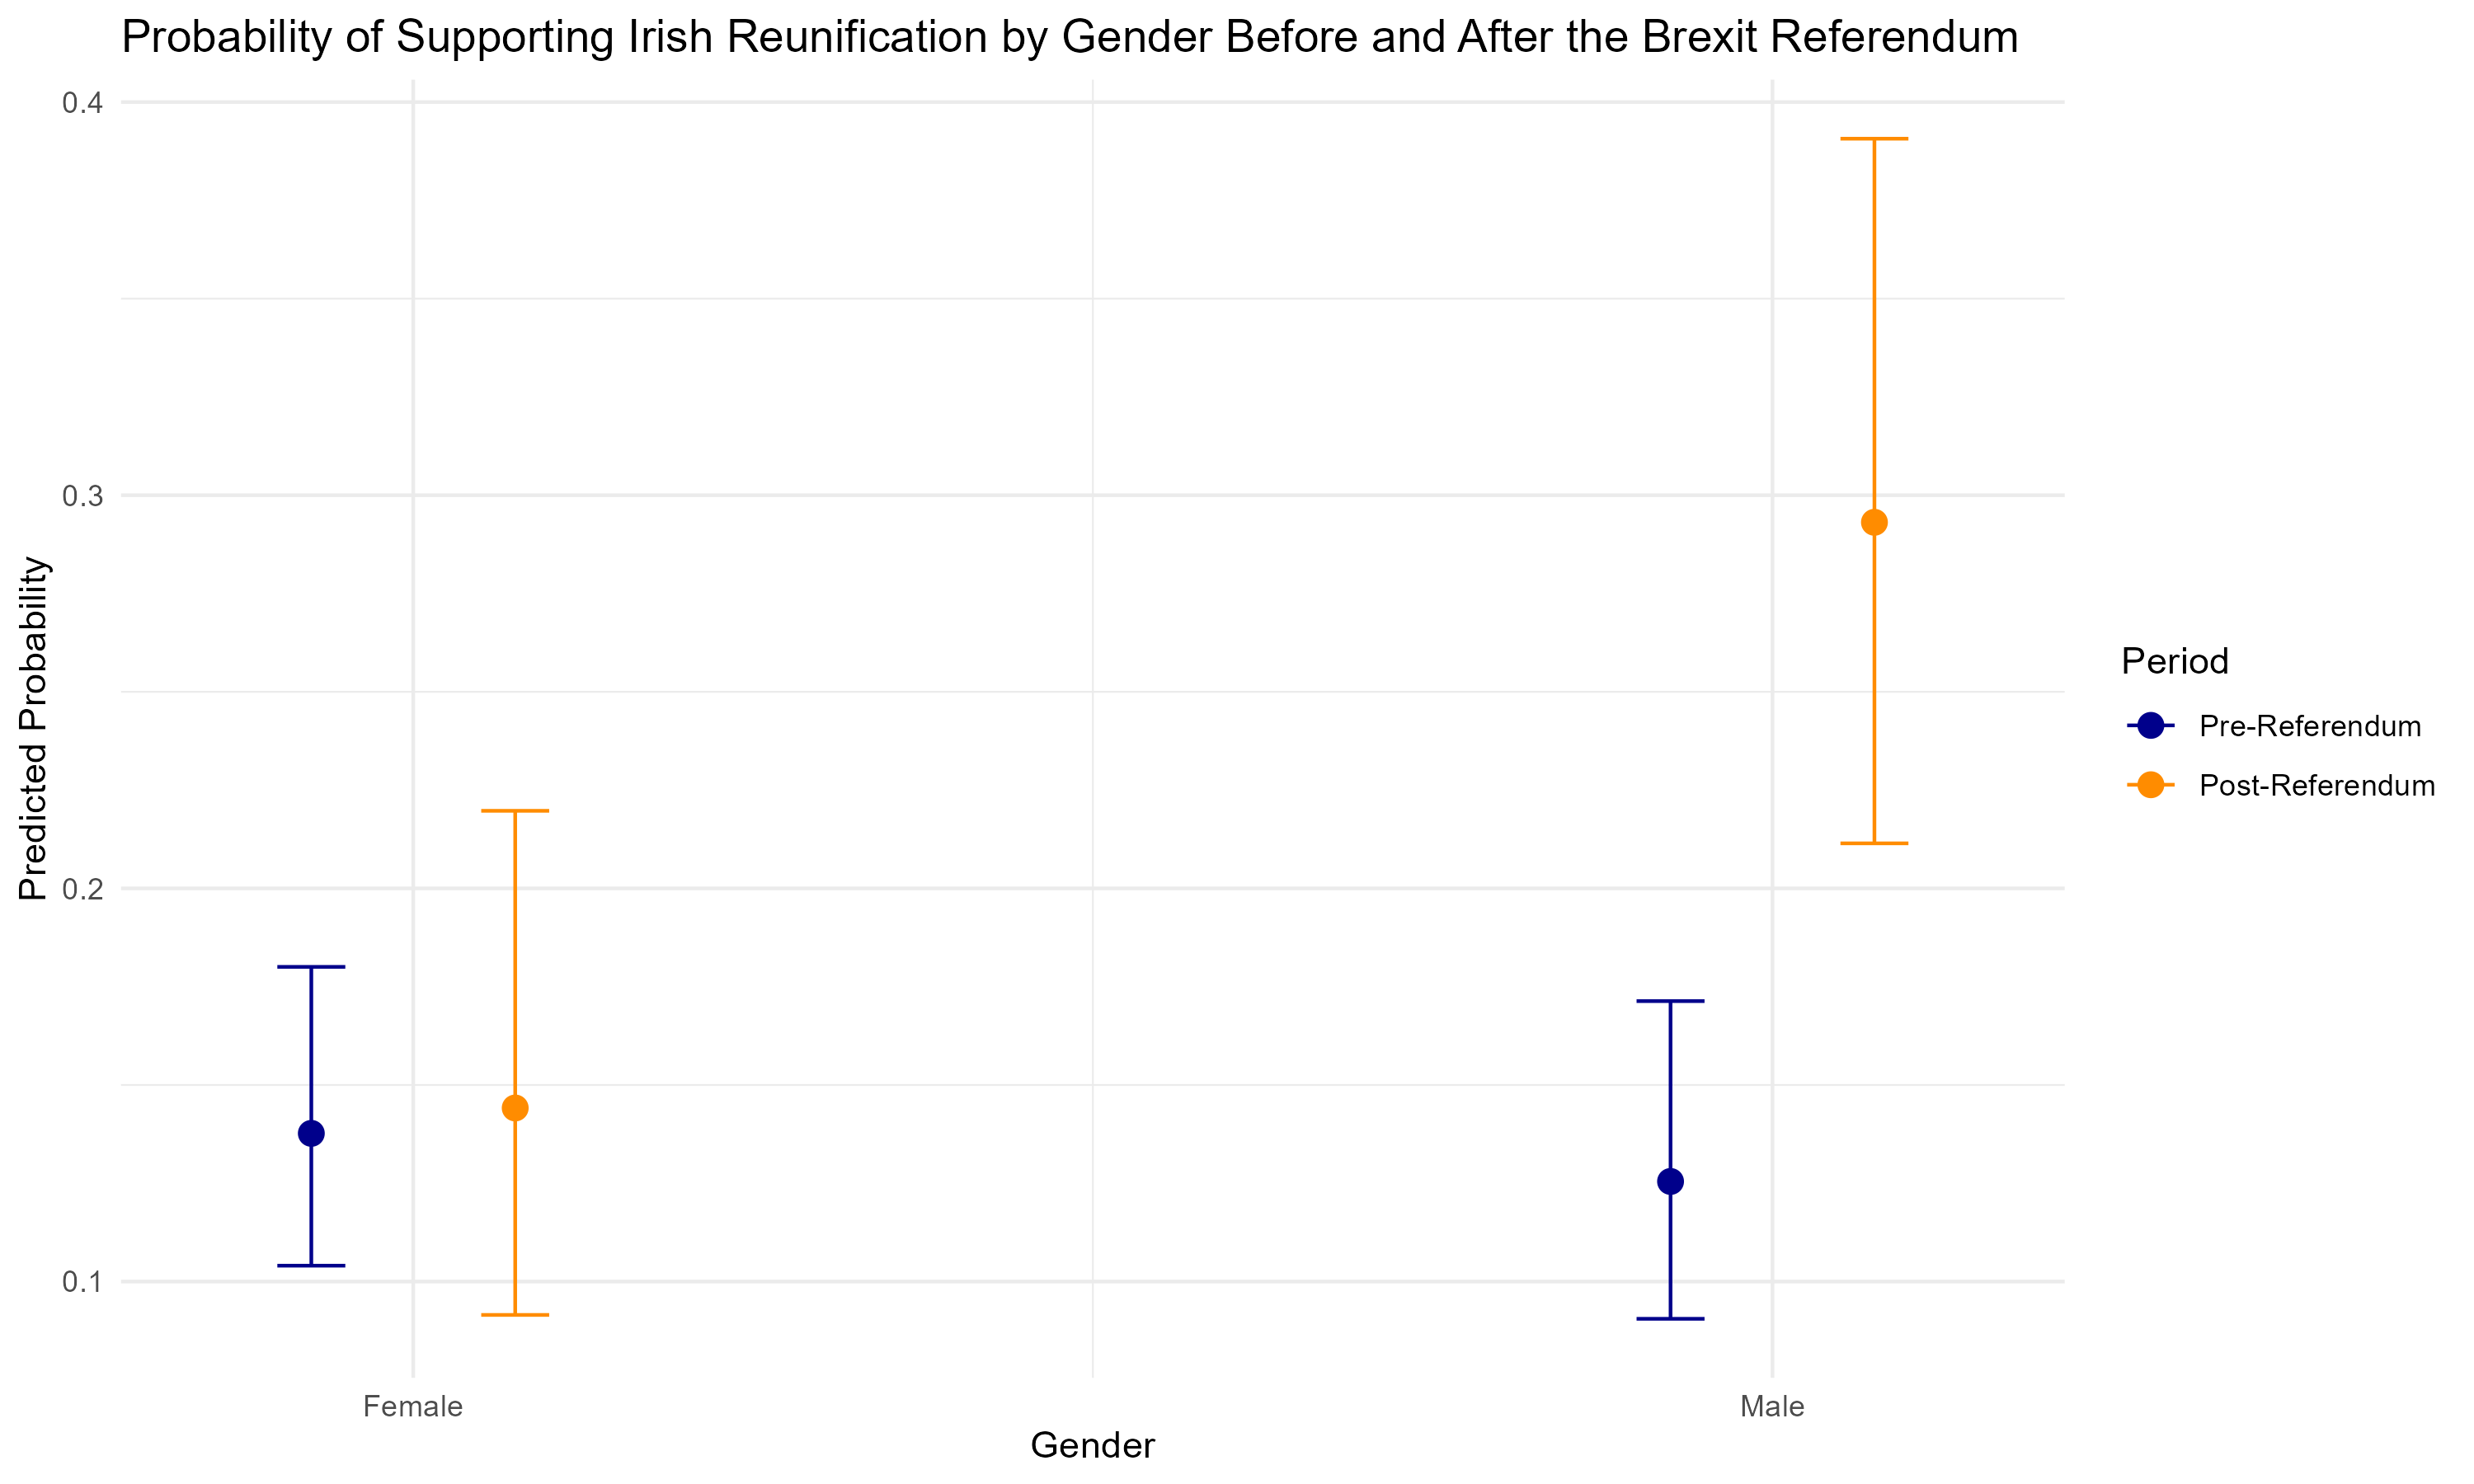
\includegraphics[width=\textwidth]{plot_ext3.png}
			\end{column}
			\begin{column}{0.5\textwidth}
				\begin{itemize}
					\item \textbf{Result:} Significant interaction.
					\item \textbf{Interpretation:} Effect considerably stronger for \textbf{men}.
					\item Possible reasons: Risk aversion in women or stronger link between masculinity and nationalist mobilization.
				\end{itemize}
			\end{column}
		\end{columns}
	\end{frame}
	
	\begin{frame}{Conclusions}
		\begin{itemize}
			\item The replication confirms the robust impact of the Brexit shock on Northern Irish public opinion.
			\item \textbf{Contribution:} My extension shows that the effect was not socially neutral:
			\begin{itemize}
				\item It is \textbf{gendered} (stronger in men).
				\item It is \textbf{trauma-sensitive} (stronger in victims).
				\item But it is \textbf{generationally homogeneous} in its reaction.
			\end{itemize}
		\end{itemize}
	\end{frame}
	
	\begin{frame}[allowframebreaks]{Bibliography}
\printbibliography
	\end{frame}
	
\end{document}